\chapter{Vergleich eines Flächenflugzeugs mit dem Quadrocopter}
\label{chap:vergleich}
Jedes Luftfahrzeugkonzept entzieht sich einem direkten Vergleich mit einem Luftfahrzeug einer anderen Art. So weist jedes Fluggerät in seiner Gattung spezifische Vorteile auf wie der Start auf der Stelle und das Hovern in der Luft für Multicopter oder der Gleitflug für Flächenflugzeuge. Die jeweilige Auslegung beider führt zu unterschiedlichen Designs was die Propeller, die Motorleistung und das -gewicht, die Größe, das Gesamtgewicht etc. betrifft. Aus diesem Grund müssen Kriterien für eine Vergleichbarkeit vorgeschrieben werden. Hierfür wird das Design des Multicopters auf das aus \cite{Anderson.2018} festgelegt, welches genauer in Kapitel \ref{sec:komponenten} beschrieben ist. Da die Flugleistungen von \cite{Anderson.2018} bekannt sind und der Quadrocopter durchaus schon im Rahmen der Anforderungen für diese Mission als optimiert betrachtet werden kann, bedarf es an dieser Stelle einer Untersuchung des Flächenflugzeuges. Dazu wird das Flächenflugzeug auf Parameter fixiert, mit denen es bereits sehr hoch aufsteigen kann. Zur Untersuchung und Vergleichbarkeit werden die Gesamtmassen beider Fluggeräte gleichgesetzt \ensuremath{m_{ges,Quadrocopter} = m_{ges,Flächenflugzeug}}. Dabei setzt sich die Masse der Flächenflugzeugbatterie   
\begin{equation}
	m_{Bat,Fl} = m_{Bat,Quad} + (m_{Mot,Quad}\cdot n_{Prop,Quad} - m_{Mot,Fl}\cdot n_{Prop,Fl}) - (1-f_P)\cdot m_{Quad}  
\end{equation}
in Bezug auf bereits gewählte Massen und auf den Quadrocopter zusammen. Der Faktor \ensuremath{f_P} kann als Penalty-Faktor verstanden werden. Dieser verringert zusätzlich die Batteriemasse, wenn das Strukturgewicht des Flächenflugzeugs das des Quadrocopters überschreitet
\begin{equation}
	f_P = \frac{m_{Flugzeug}}{m_{Quad}} \eqend{.}
	\label{eq:penalty}
\end{equation} 
Für eine erste Betrachtung wird der Penalty-Faktor auf 1 gesetzt. Dies entspricht einer optimistischen Einschätzung. Im Anschluss werden die Parameter in näherer Umgebung der ersten festgesetzten Werte variiert. Dadurch kann der Einfluss auf das Leistungsverhalten und die Richtung der möglichen Optimierung bestimmt werden. Diese erste, einfache Untersuchung ist nur eine sehr oberflächliche, weil jeder Parameter nur einzeln und unabhängig von den anderen untersucht wird. Jegliche Kombinationen von Einflüssen wie der Einfluss der Masse auf die Steiggeschwindigkeit oder vergleichbare Beziehungen werden vernachlässigt. Im Hinblick auf diese erste, kleine Optimierung ist der Kostenfaktor die maximal erreichbare Höhe beider Fluggeräte. Je nachdem welches der beiden Fluggeräte effektiver und effizienter eine maximale Flughöhe erreicht, wird es weiter untersucht und anschließend optimiert.  

\section{Einfluss der Steiggeschwindigkeit auf den Quadrocopterflug}
Bevor ein Vergleich zwischen dem Flächenflugzeug und dem Quadrocopter aus Kap. \ref{chap:chap:nachbildung_des_quadrocopter} durchgeführt werden kann, muss noch die Steiggeschwindigkeit für den Quadrocopter optimiert werden. \\
Für das Flächenflugzeug werden für jeden Höhenschritt, wie bereits in Abschn. \ref{subsubsec:schub_flaechenflzg} dargelegt, der Bahnneigungswinkel und die Fluggeschwindigkeit optimiert. Dies entspricht einer ersten Optimierung. Dabei wird der Bahnneigungswinkel für jeden Höhenschritt iteriert. Die Fluggeschwindigkeit berechnet sich in Abhängigkeit vom Bahnneigungswinkel (vgl. Gleichung \eqref{eq:eq:geschw_flaechenflugzeug}). Die Auswahl erfolgt anhand der minimalen Energiemenge, die der Batterie für den Höhenschritt entnommen wird. Analog dazu, erfolgt auch die Optimierung der Steiggeschwindigkeit des Quadrocopters (vgl. Anhang \ref{sec:vvar_vorgehen}). \\
Durch die Optimierung der Steiggeschwindigkeit ist ein zusätzlicher Höhengewinn von \SI{1000}{m} im Vergleich zu dem Flug mit konstanter Bahngeschwindigkeit von \SI{10}{m/s} zu vermerken. Bei dem neuen TOC auf \SI{14100}{m} wird allerdings die sogenannte Dienstgipfelhöhe erreicht (genauere Beschreibung in Abschn. \ref{sec:flaechenflugzeug_referenzkonfig} und \ref{subsec:mot_prop_kombi}). Ohne diese Limitierung und bei linearer Extrapolation Restladungskurve könnte der Quadrocopter bei Verwendung eines anderen Propellers eine Höhe von \SI{17000}{m} erreichen. Die Flugleistungen sind nicht durch die Motorleistung begrenzt, sondern durch die Maximaldrehzahl des Propellers. Diese liegt bei \SI{17000}{RPM}. Ein Grund dafür kann in der Festigkeit des Propellers gefunden werden. Nichtsdestotrotz ist ein Flug mit variierbarer Steiggeschwindigkeit signifikant effizienter. Dies macht sich deutlich in der Restladung bemerkbar. Die Abnahme der Restladung ist pro Höhenschritt geringer als in Kap. \ref{sec:ergebnisse_quadrocopter}. Auf \SI{10260}{m} sind noch \SI{40}{\%} Restladung vorhanden. Das entspricht ca. \SI{10}{\%} mehr Restladung in der gleichen Höhe wie in Kap. \ref{chap:nachbildung_des_quadrocopter}. Die Propellerdrehzahl steigt beinahe sofort auf ihr Maximum von \SI{17000}{RPM} an und verbleibt auf diesem Niveau bis zum TOC. Rückwirkend ist damit auch der Motorstrom ab \SI{4000}{m} auf dem Niveau der Batteriespannung und somit die PWM auf \SI{100}{\%}. Der Leistungsüberschuss ist gleich null. Dieser Zustand ist auch durch ein Maximum der Bahngeschwindigkeit gekennzeichnet mit \SI{30}{m/s}. Die Bahngeschwindigkeit ist damit dreimal so hoch wie die vorherigen \SI{10}{m/s}. Der Motorstrom \ensuremath{I_{Mot}} sinkt im Laufe des Fluges immer weiter ab. Da die Drehzahl konstant bleibt, die Dichte aber mit der Höhe abnimmt, sinkt auch das Drehmoment an der Motorwelle und letztlich der Motorstrom (vgl. Gleichung \eqref{eq:motorstrom}). Über den Motorstrom sinkt die Motorspannung ebenfalls leicht ab (vgl. Gleichung \eqref{eq:motorspannung}), weil die Drehzahl auf einem konstanten Niveau bleibt. Während die Batteriespannung von \SI{16}{V} auf \SI{15}{V} durch die Last einbricht, fällt mit der Motorspannung auch die PWM unterhalb von \SI{100}{\%} ab. Die Bahngeschwindigkeit steigt zuerst auf ihr Maximum, sinkt danach aber kontinuierlich auf \SI{0}{m/s}. Somit wird die Dienstgipfelhöhe erreicht. Die Flugzeit kann auf die Bahngeschwindigkeit zurückgeführt werden. Bereits nach \SI{13}{min} und \SI{20}{sec} wird der TOC erreicht. \\
Der Motorregler verzeichnet wenige Verluste durch die hohe PWM und besitzt deshalb einen hohen Wirkungsgrad. Der Propellerwirkungsgrad steigt am Anfang durch den Drehzahlanstieg (vgl. Gleichung \eqref{eq:eta_prop}) und ebenso mit dem Schub und der Bahngeschwindigkeit. Während der Schubüberschuss aufgebraucht ist, sinkt mit der Höhe die Dichte und dementsprechend der Schub. Mit dem Schub sinkt auch die leistungstechnisch mögliche Bahngeschwindigkeit, was einen starken Einbruch im Propellerwirkungsgrad hervorruft.

\begin{figure}[htb!]
\centering
	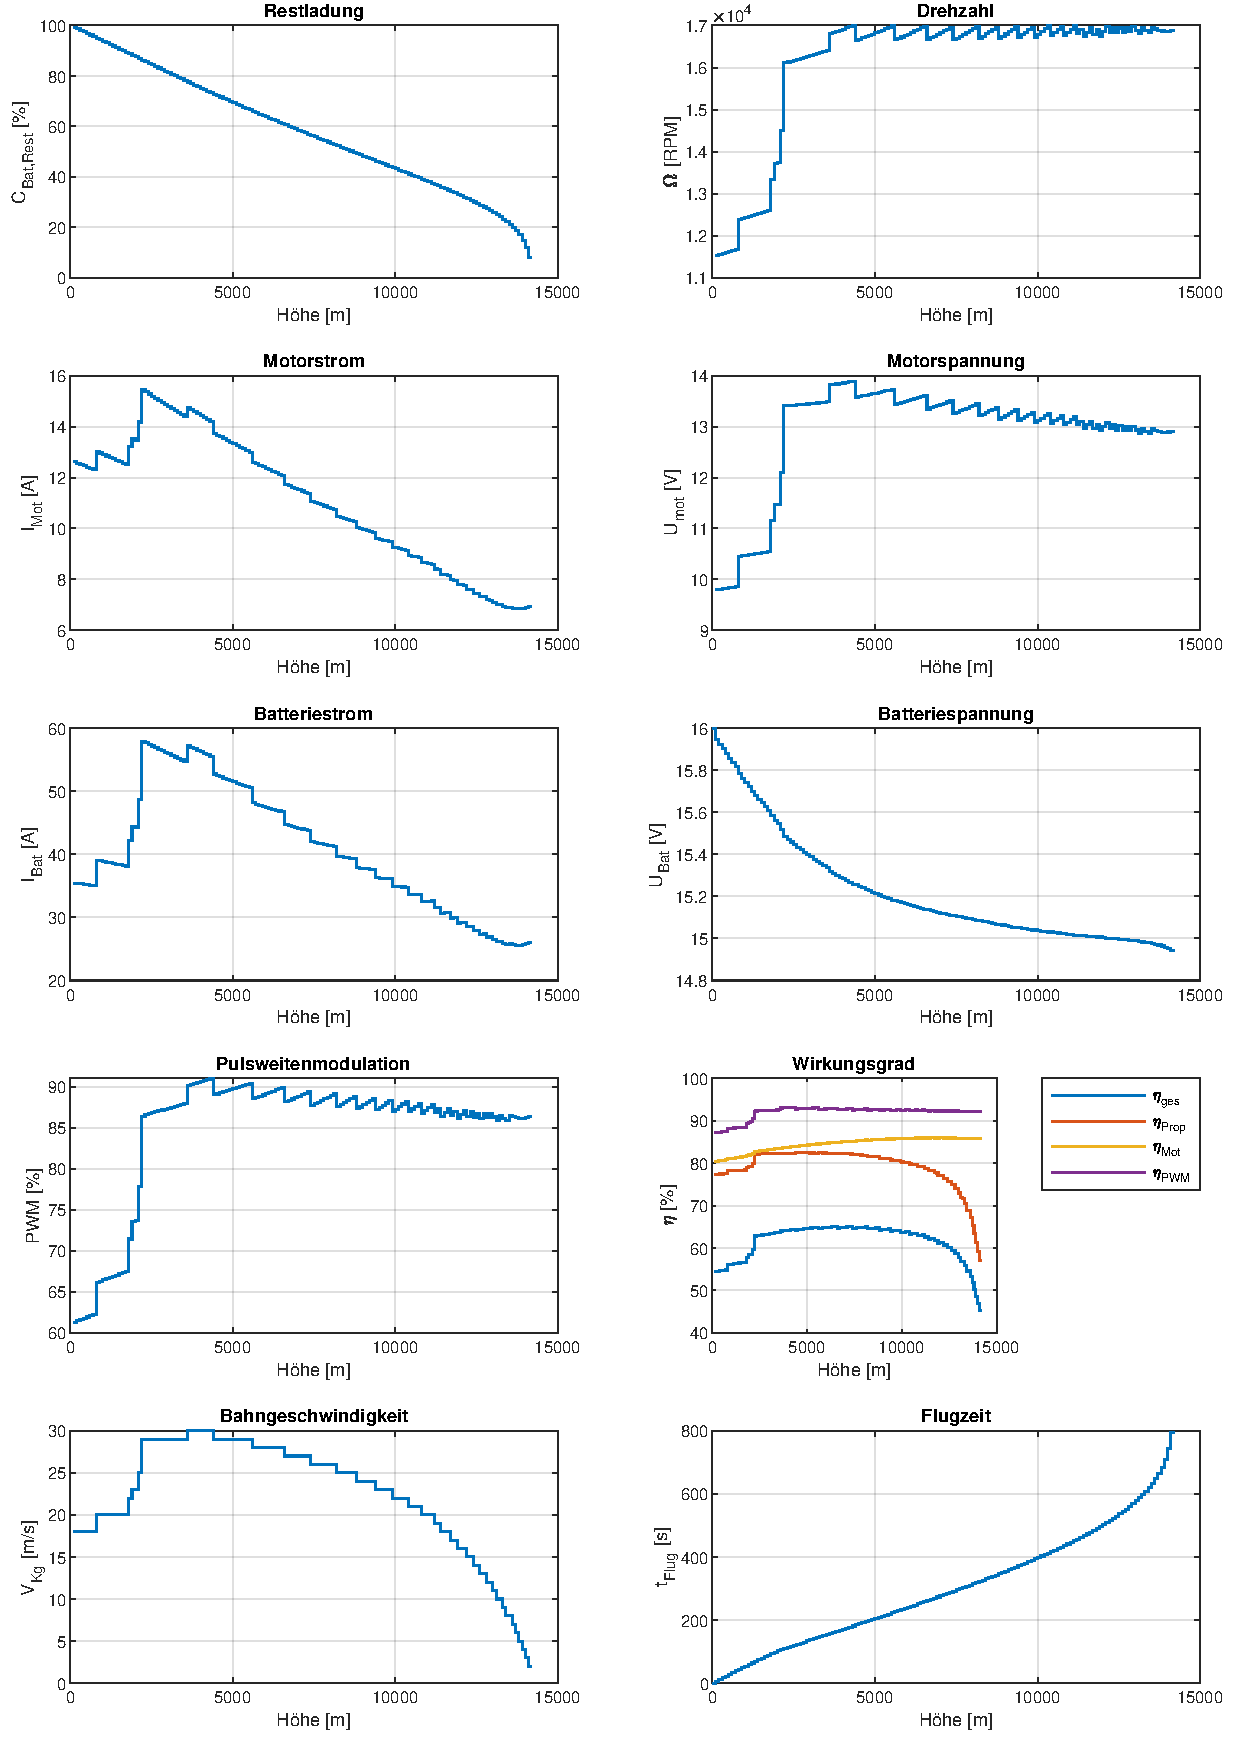
\includegraphics[scale=0.7]{Diagramme/Russland_vvar.pdf}
	\caption{Flugleistungen des Quadrocopter aus \cite{Anderson.2018} mit variabler Steiggeschwindigkeit}
	\label{abb:russland_vvar}
\end{figure}



\section{Flächenflugzeug-Referenzkonfiguration}
\label{sec:flaechenflugzeug_referenzkonfig}
In der Tab. \ref{tab:referenzkonfiguration} sind wichtige Parameter der Referenzkonfiguration für das Flächenflugzeug aufgelistet. Die Werte wurden in ersten Untersuchungen durch Versuche bestimmt. 
\begin{center}
	\captionof{table}{wichtige Parameter der Flächenflugzeug-Referenzkonfiguration}
	\begin{tabular}{l l l} \hline
		Parameter & Variablenname & verwendete Größe \\ \hline
		Leermasse des Flächenflugzeug \ensuremath{m_{Flugzeug}}& \texttt{m\_Flugzeug} & \SI{0,354}{kg} \\ 
		Batteriemasse \ensuremath{m_{Bat}} & \texttt{m\_Bat} & \SI{0,56}{kg} \\
		Motormasse \ensuremath{m_{Mot}}& \texttt{m\_Mot} & \SI{0,106}{kg} \\
		Geschwindigkeitskonstante \ensuremath{K_V} & \texttt{K\_V} & \SI{1390}{RPM/V} \\
		maximaler Dauerstrom \ensuremath{I_{max}} & \texttt{I\_max} & \SI{35}{A} \\
		Propeller & \texttt{prop\_name} & 9x7 \\
		Anzahl Propeller \ensuremath{n_{Prop}} & \texttt{n\_prop} & \SI{1}{} \\
		Auslegungsgleitzahl \ensuremath{E^{\star}} & \texttt{E\_stern} & \SI{4}{} \\
		Auslegungsgeschwindigkeit \ensuremath{V^{\star}} & \texttt{V\_stern} & \SI{100}{km/h} \\
		Gleitzahl \ensuremath{E} & \texttt{E} & \SI{4}{} \\ 
		Anzahl der Batteriezellen \ensuremath{N_{Bat,cell}} & \texttt{N\_bat\_cell} & 6 \\	
		Penalty-Faktor \ensuremath{f_P}	& \texttt{f\_P}	& 1 \\ \hline
	\end{tabular}	
	\label{tab:referenzkonfiguration}
\end{center}
Diese Konfiguration ist die Grundlage aller Untersuchungen, die das Flächenflugzeug betreffen.



\begin{figure}[htb!]
%\centering
	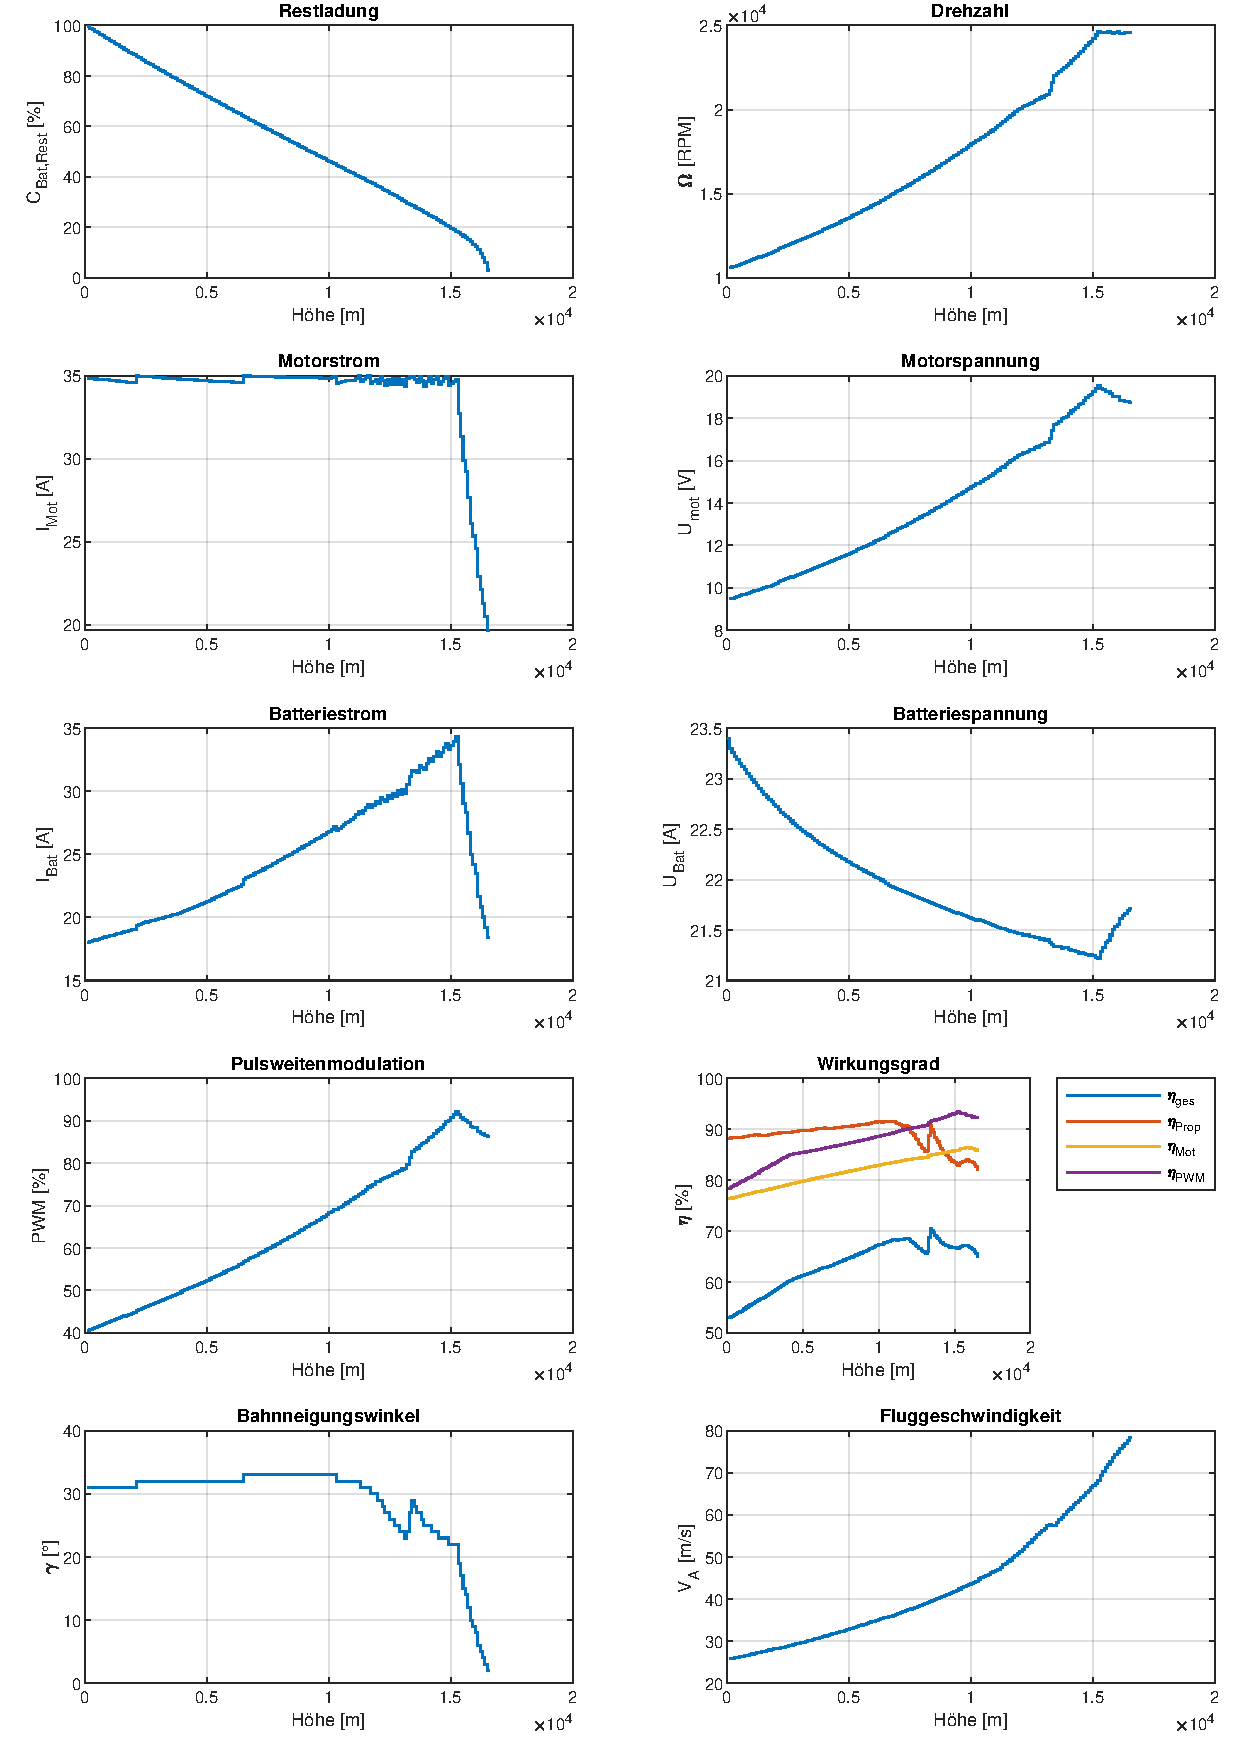
\includegraphics[scale=0.7]{Diagramme/Ausgangskonstellation.pdf}
	\caption{Verlauf der Leistungsparameter über der Höhe für die Flächenflugzeug-Referenzkonfiguration (Tab. \ref{tab:referenzkonfiguration})}
	\label{abb:referenzkonfiguration}
\end{figure}
Die in Tab. \ref{tab:referenzkonfiguration} beschriebene Referenzkonfiguration erreicht bereits eine Flughöhe von \SI{16500}{m}. Der limitierende Parameter für den Aufstieg in noch größere Höhen ist in diesem Fall nicht die Motorleistung, sondern die maximale Propellerdrehzahl (vgl. Abb. \ref{abb:referenzkonfiguration}). Eine weitere Erhöhung der Drehzahl ist in diesem Fall wegen folgender zwei Einflussfaktoren nicht möglich. Zum einen ist die maximale Propellerdrehzahl auf \SI{25000}{RPM} durch das Ende des Kennfeldes begrenzt. Dies ist mit hoher Wahrscheinlichkeit auf die Festigkeit des Propellers zurückzuführen. Bis zu dieser Drehzahl ist ein uneingeschränkter Betrieb des Propellers möglich, ohne das ein strukturelles Versagen des Propellers zu befürchten ist. Ab einer höheren Drehzahl kann ein sicherer Betrieb nicht mehr gewährleistet werden. Der zweite Einflussfaktor ist die Blattspitzengeschwindigkeit \ensuremath{Ma_{tip}}. Diese erreicht ab \SI{15000}{m} Höhe \ensuremath{Ma_{tip} = 1}. Damit kommt es zu Machzahleffekten und einer relativen Überschallanströmung an der Propellerblattspitze. Die dadurch verursachten zusätzlichen Verluste (z.B. Stoßverluste), Stömungsablösungen, Verminderungen in der Schuberzeugung usw. können nicht in dem einfachen Luftmodell berücksichtigt werden, das dem in Kap. \ref{chap:Programmbeschreibung} erläuterten Programm zur Flugleistungsberechnung zugrunde gelegt wurde. An dieser Stelle können transsonische Effekte, die bereits bei einer relativen Anströmung an der Propellerspitze von \ensuremath{Ma < 1} auftreten können, nicht ausgeschlossen werden. Die Möglichkeiten zur Vermeidung dieser Begrenzung werden in Abschn. \ref{subsec:propeller} beschrieben. \\
Die Limitierung der Flughöhe durch die maximale Propellerdrehzahl stellt eine sogenannte Dienstgipfelhöhe dar. Diese limitiert den Steigflug bereits zu Beginn des Starts auf \SI{16500}{m}. Eine Erhöhung der Motorleistung, der Batteriezellenanzahl oder beispielsweise der Kapazität würde keine weiteren Verbesserungen der Flugleistungen erbringen, da die Begrenzung durch die Propellerdrehzahl für jeden Flug dieselbe ist. Generell ist eine Erhöhung des Leistungsüberschuss (\ensuremath{=} Erhöhung der Leistung) damit nicht zielführend. Ein Steigflug ohne Dienstgipfelhöhe zeichnet sich durch die Limitierung der Flughöhe durch die Restladung aus. Hierbei sinkt diese linear ab bis \SI{0}{\%} Restladung erreicht sind. \\
Das Erreichen der Dienstgipfelhöhe zeichnet sich durch eine Verschlechterung Flugleistungen aus. Die Restkapazität nimmt mit der Höhe linear ab. Ab der Höhe von \SI{15000}{m} wird die maximale Propellerdrehzahl erreicht, sodass sich die Abnahme der Restkapazität erhöht. \\
Der Steigflug bis \SI{15000}{m} ist durch den Betrieb bei maximalem Dauerstrom (\ensuremath{I_{max} = \SI{35}{A}}) gekennzeichnet. Dadurch stellt sich ein optimaler Bahnneigungswinkel von \SI{31}{^\circ} bis \SI{33}{^\circ} ein. Dieser Winkel kann bis zu einer Höhe von \SI{10000}{m} gehalten werden, bevor er zunächst langsam absinkt und ab \SI{15000}{m} steil gegen \SI{0}{^\circ} strebt. Die Fluggeschwindigkeit steigt mit dem Steigwinkel progressiv mit dem Produkt aus \ensuremath{\sqrt{\rho^\star/\rho}} an (vgl. Gleichung \eqref{eq:geschw_flaechenflugzeug}). \\
Zu Beginn des Steigfluges wären größere Steigwinkel effizienter, allerdings werden diese durch den maximalen Motorstrom \ensuremath{I_{max}} begrenzt. Ohne diesen würde der Bahnneigungswinkel beinahe linear absinken. Daraus kann geschlossen werden, dass ein Flug mit maximalem Motorstrom im unteren Höhenbereich am effizientesten ist. Der sägezahnartige Verlauf des Motorstroms hängt mit der gewählten Diskretisierung und dadurch rückwirkend mit der Genauigkeit der Berechnung zusammen. Eine genauere Untersuchung der in den Diagrammen dargestellten Punkte und deren Umgebung würde zu einem glatten Verlauf des Motorstroms bei \ensuremath{I_{max}} führen. Ebenso würden sich die Verläufe aller anderen Leistungsparameter über der Höhe glätten. Gleichzeitig zum konstanten Motorstrom wächst die Motorspannung linear an, bis diese ab \SI{9800}{m} das Niveau der Batteriespannung erreicht. \\
Auch die Propellerdrehzahl weist eine progressive Zunahme auf. Mit der Höhe sinkt die Dichte der Luft entsprechend nach Gleichung \eqref{eq:rho_0_11} und \eqref{eq:dichte_strato}. Zur Erzeugung des gleichen Schubs muss mit der abnehmenden Dichte die Drehzahl steigen, um den Massenstrom durch die Propellerebene und letztendlich den Schub konstant zu halten (vgl. Gleichung \eqref{eq:propellerschub}). Bei konstantem Motorstrom und steigender Propellerdrehzahl nimmt entsprechend auch die Motorspannung zu (vgl. Gleichung \eqref{eq:motorspannung}). \\
Der Verlauf des Batteriestroms steht in direktem Zusammenhang mit dem Motorstrom und der Motorspannung. Dies wird aus Gleichung \eqref{eq:batteriestrom} ersichtlich. Bei einem konstantem Motorstrom ist  \ensuremath{I_{Bat}} nur von \ensuremath{U_{Mot}} abhängig. Daher zeigt sich der gleiche Verlauf wie bei \ensuremath{U_{Mot}}. Ab dem Erreichen der maximalen Propellerdrehzahl nimmt \ensuremath{U_{Mot}} wieder leicht ab und \ensuremath{I_{Bat}} hängt nur noch von \ensuremath{I_{Mot}} ab. Der Verlauf der Drehzahl ist ausschlaggebend für die Motorspannung. Die Batteriespannung bricht durch die Belastung von anfänglichen \SI{23,4}{V} auf \SI{21,2}{V} ein. 
Die PWM steigt mit dem Verlauf der Motorspannung sowie der Batteriespannung an. Ab \SI{15000}{m} erreicht sie ihr Maximum bei \SI{91,5}{\%}. Dies verdeutlicht noch einmal, dass für die Referenzkonfiguration die Motorleistung nicht den die Höhe limitierenden Leistungsparameter darstellt. \\
Ist die maximale Propellerdrehzahl ab \SI{15000}{m} erreicht, fällt der Motorstrom rapide mit der konstanten Drehzahl ab. Da die Drehzahl konstant bleibt bis zum TOC, nimmt das Propellerdrehmoment und damit auch der Motorstrom mit zunehmender Höhe und abnehmender Dichte ab (vgl. \eqref{eq:motorstrom}). Mit sinkendem Motorstrom sinkt auch die Motorspannung  (vgl. Gleichung \eqref{eq:motorspannung}) und schließlich die PWM (vgl. Gleichung \eqref{eq:pwm}). Dieser Effekt wird noch durch den Anstieg der Batteriespannung auf \SI{21.7}{V} verstärkt. Der sinkende Propellerschub bei konstanter Drehzahl hat außerdem ein Sinken des Bahnneigungswinkels \ensuremath{\gamma} zur Folge. Der sinkende Schub reicht für größere Bahnneigungswinkel nicht mehr aus. Mit diesem Absinken der Restladung und des Bahnneigungswinkel gegen null ist die Dienstgipfelhöhe erreicht, ab der kein weiterer Steigflug mehr möglich ist. Jedoch würde auch ohne diese Begrenzung der TOC nur ein paar hundert Meter höher liegen, wenn die Restladungskurve linear extrapoliert würde. \\
Der schnelle und deutliche An- und Ab-stieg im Bahnneigungswinkel, der sich durch alle anderen Diagramme fortpflanzt, kann auf eine Inkonsistenz im Kennfeld oder Berechnungsfehler zurückverfolgt werden.\\
Der Gesamtwirkungsgrad gliedert sich wie in Kap. \ref{subsec:eta_ges} dargelegt in den Propeller-, den Motor- und den Motorreglerwirkungsgrad. Daher folgt er zeitgleich den anderen Wirkungsgraden. Der Propellerwirkungsgrad steigt mit der Höhe an. Ausschlaggebend hierfür ist die steigende Geschwindigkeit und die Drehzahl (vgl. Gleichung \eqref{eq:eta_prop}). Während der Bahnneigungswinkel ab \SI{10000}{m} abfällt, steigt die Bahngeschwindigkeit und der Propellerwirkungsgrad. Über Gleichung \eqref{eq:geschw_flaechenflugzeug} nimmt mit steigendem Bahnneigungswinkel die Fluggeschwindigkeit ab. Da dieser jedoch nun absinkt, nimmt damit im Umkehrschluss die Fluggeschwindigkeit zu. \\
Da die Motorspannung bereits ihr Maximum erreicht hat, kann die Propellerdrehzahl nur noch leicht mit der abnehmenden Dichte und somit geringer werdenden Widerstandskräften ansteigen (vgl. Gleichung \eqref{eq:motorspannung}). Dabei nimmt auch das Propellerdrehmoment ab (Ergebnis aus Gleichung \eqref{eq:motorstrom}). Bei einer gleichermaßen steigenden Fluggeschwindigkeit steigt die Strahlleistung des Propellers (vgl. Gleichung \eqref{eq:strahlleistung}). Als Konsequenz steigt der Propellerwirkungsgrad.
Dies gilt auch für den Motorwirkungsgrad. Dieser steigt mit wachsender Propellerdrehzahl und -drehmoment (vgl. Gleichung \eqref{eq:eta_mot}). Außerdem nehmen die durch den Innenwiderstand und den Leerlaufstrom verursachten Verluste anteilig am Motorstrom und der -spannung ab (vgl. Gleichung \eqref{eq:motorstrom} und \eqref{eq:motorspannung}). Der Grund hierfür liegt in der Annahme, dass diese beiden Motorkenngrößen für jeden Motorzustand als konstant angesehen werden. Der Wirkungsgrad des ESC steigt simultan mit der Höhe und der PWM. Mit steigender PWM nehmen auch die Verluste innerhalb des Motorreglers ab (vgl. Gleichung \eqref{eq:eta_pwm}). Deutlich zu erkennen ist eine leichte Abnahme aller Wirkungsgrade ab \SI{15000}{m}. Der Propellerwirkungsgrad nimmt dabei deutlich schneller ab. Die Begründung kann in dem abnehmenden Schub und die mit konstanter Drehzahl abnehmende induzierte Geschwindigkeit gefunden werden. Dies ist ein Indiz für den Beginn eines ineffizienteren Flugzustandes.



\section{Einflussfaktoren auf das Flächenflugzeug}
Die zu variierenden Parameter des Flächenflugzeugs sind diejenigen Leistungsparameter, die das Fluggerät qualifizieren. Das sind die Motor-Propeller-Kombination, die Propelleranzahl, die Gleitzahl, die Auslegungsgeschwindigkeit und der Penalty-Faktor.

\subsection{Propeller}
\label{subsec:propeller}
Wie in Abschn. \ref{subsec:flugleistungen_flaechenflugzeug} ersichtlich wird, kann die Propellerdrehzahl und insbesondere die Blattspitzengeschwindigkeit die Flugleistungen limitieren. Für eine vorgegebene Fluggerätekonfiguration kann die Propellerdrehzahl nicht direkt beeinflusst werden, weil die Schubanforderung die Drehzahl bestimmt. Eine Möglichkeit indirekt Einfluss zu nehmen ist über den Propeller an sich. Die veränderbaren Propellerparameter sind die Propellersteigung und der Propellerdurchmesser. 
Zum einen kann ein Propeller mit größerer Steigung gewählt werden. Mit der größeren Steigung ist es möglich denselben Schub bei verringerter Drehzahl zu erzeugen. Die andere Möglichkeit umfasst eine Vergrößerung des Propellerdurchmessers. Hierfür gilt derselbe Zusammenhang wie für die Propellersteigung. Entsprechend steigt auch die Effizienz \cite[119]{Wall.2015}.


\subsection{Motor-Propeller Kombination}
\label{subsec:mot_prop_kombi}
Die Motor-Propeller-Kombination beeinflusst entscheidend das Leistungsverhalten von elektrischen, propellergetriebenen Fluggeräten. Mit dem in Tab. \ref{tab:referenzkonfiguration} aufgeführten Motor mit einem Gewicht von \SI{106}{g} und einem \ensuremath{K_V}-Wert von \SI{1390}{RPM/V} sind bereits sehr hohe Flughöhen erreichbar. Bei Verwendung des gleichen Propellers, einem 9x7 Propeller, und einer Variation des Motors mit einem anderen \ensuremath{K_V}-Wert, zeigen die Motoren mit einem größeren \ensuremath{K_V}-Wert ein höhere Dienstgipfelhöhe (vgl. Abb. \ref{abb:flaechenflzg_mot_prop}). Alle Motoren bis auf den mit einem \ensuremath{K_V}-Wert von \SI{2850}{RPM/V} erreichen eine entsprechende Dienstgipfelhöhe.\\
Über die Betrachtung der Restladung kann die Effizienz der Motoren am besten beurteilt werden. Hier verzeichnet der Motor mit einem \ensuremath{K_V}-Wert von \SI{2850}{RPM/V} die schlechtesten Flugleistungen, da die Restladung am stärksten abnimmt und schon bei \SI{10000}{m} \SI{0}{\%} erreicht. Bei den Motoren mit einem \ensuremath{K_V} von \SI{1390}{RPM/V} und \SI{1640}{RPM/V} sind die Unterschiede marginal. Die Dienstgipfelhöhe ist in etwa dieselbe bei ca. \SI{16500}{m} Höhe. Der \SI{1390}{} \ensuremath{K_V} Motor weist bei genauerer Betrachtung jedoch eine leicht verbesserte Effizienz auf, da die Restladung in jedem Höhenschritt höher ist. \\
Deutlich geringere Dienstgipfelhöhen als die beiden zuvor erwähnten Motoren weisen die Motoren mit einem \ensuremath{K_V}-Wert von \SI{840}{RPM/V} und \SI{1035}{RPM/V} auf. Allerdings ist die Effizienz in jedem Höhenlevel gegenüber allen anderen Motoren höher. Der Verlauf der beiden Restladungskurven ist bis \SI{10000}{m} identisch bevor der Motor mit dem geringeren \ensuremath{K_V} bei \SI{12000}{m} und der mit der mit dem höheren bei \SI{15000}{m} seine Dienstgipfelhöhe erreicht. 
An dieser Stelle sei nochmal auf den Begriff der Dienstgipfelhöhe hingewiesen. Diese zeichnet sich durch eine Limitierung des TOC infolge der fehlenden Antriebsleistung zum Aufstieg in noch größere Flughöhen aus (vgl. Abschn. \ref{sec:flaechenflugzeug_referenzkonfig}). Kennzeichnend für diesen Flugzustand ist das vollständige Aufbrauchen des Leistungsüberschuss. Trotzdem gilt für alle Fluggeräte der Flug mit maximalem Motorstrom bei einem noch vorhandenen Leistungsüberschuss am effizientesten.
Die Motoren mit einem \ensuremath{K_V} von \SI{1390}{RPM/V} und \SI{1640}{K_V} weisen das gleiche Flugverhalten auf, das in Abschn. \ref{sec:flaechenflugzeug_referenzkonfig} beschrieben wird.
Mit dem \ensuremath{K_V}-Wert steigt ebenso die Dienstgipfelhöhe (vgl. Abb. \ref{abb:flaechenflzg_mot_prop}). Den größten Einfluss hat der \ensuremath{K_V}-Wert auf die Motorspannung. Hier gilt, dass bei einer annähernd gleichen Drehzahl die Motorspannung mit dem \ensuremath{K_V}-Wert sinkt. Der Grund dafür liegt in der Definition dieses Motorkennwertes.\\

\begin{figure}[htb!]
\centering
	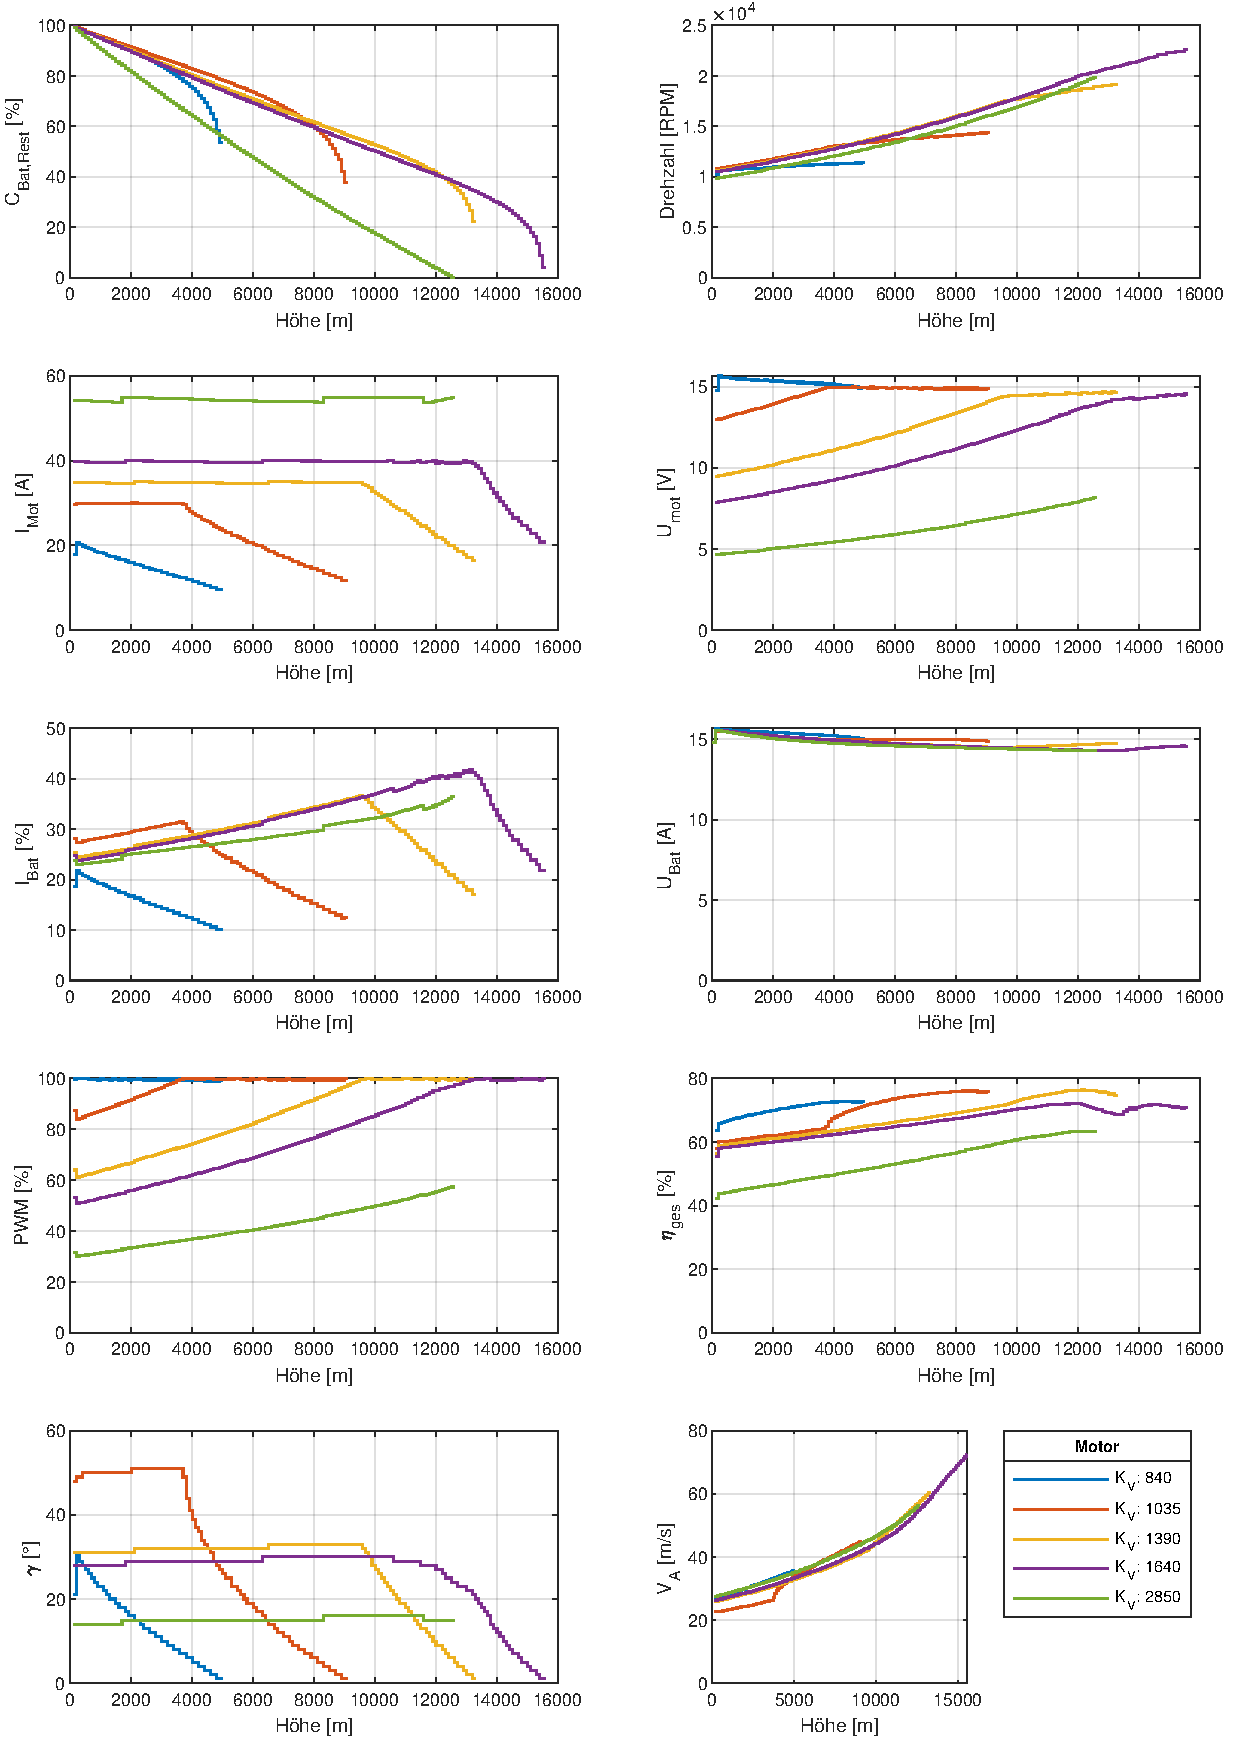
\includegraphics[scale=0.7]{Diagramme/Flaechenflzg_Mot_Prop.pdf}
	\caption{Einfluss der Motor-Propeller-Kombination auf die Flugleistungen der Flächenflugzeug-Referenzkonfiguration (Tab. \ref{tab:referenzkonfiguration})}
	\label{abb:flaechenflzg_mot_prop}
\end{figure}

Der \ensuremath{K_V}-Wert ist ein Kennwert für die Anzahl der Umdrehungen pro Minute pro Volt im Leerlauf. Ein hoher \ensuremath{K_V}-Wert bedeutet nun im Umkehrschluss, dass bei einer hohen Drehzahl die Spannung geringer ist als für einen Motor mit einem vergleichsweise niedrigem \ensuremath{K_V}-Wert. Die Drehzahl ist in diesem Fall für fast alle Motoren identisch bzw. die Unterschiede minimal. Gleichzeitig sinkt allerdings das Verhältnis von Drehmoment pro Ampere, das der \ensuremath{K_M}-Wert ausdrückt  \cite[S.35 und S.42-43]{Buchi.2013}. Es gilt die Beziehung
\begin{equation}
	K_M = 1/K_V\cdot 30/\pi \eqend{.}
\end{equation}
Ein Motor mit hohem \ensuremath{K_V}-Wert muss daher einen hohen Dauermotorstrom besitzen, um gute Flugleistungen zu erzielen (vgl. Abb. \ref{abb:flaechenflzg_mot_prop}). Durch diese Abhängigkeit wird auch die PWM beeinflusst. Der Motor mit einem \ensuremath{K_V} von \SI{840}{RPM/V} erreicht durch seine hohe Motorspannung deutlich schneller das Niveau der Batteriespannung und hat somit seinen Leistungsüberschuss aufgebraucht. Somit wird auch frühzeitiger das Absinken des Bahnneigungswinkels eingeleitet. Für Motoren mit einem niedrigeren \ensuremath{K_V}-Wert bedeutet dies auch gleichzeitig das Ende des Steigfluges. \\
Dieser Zusammenhang stellt sich für Motoren mit hohem \ensuremath{K_V}-Wert dar. Hier wird \SI{100}{\%} PWM erst bei deutlich größeren Höhen erreicht oder gar nicht, weshalb folglich der optimale Bahnneigungswinkel erst in größeren Höhen nicht mehr gehalten werden kann und danach sinkt. Bei \ensuremath{\gamma = \SI{0}{^\circ}} ist der Steigflug beendet. Hierbei steigt zudem der optimale Bahnneigungswinkel mit dem \ensuremath{K_V}-Wert. Da die Geschwindigkeit mit einem höheren Bahnneigungswinkel sinkt (vgl. Gleichung \eqref{eq:geschw_flaechenflugzeug}), sinkt auch die benötigte Leistung, die hauptsächlich für die Motoren mit geringem \ensuremath{K_V} begrenzend ist. Dabei nimmt die Restladung für kleinere \ensuremath{K_V}-Werte nicht so schnell ab wie dies für große \ensuremath{K_V}-Werte der Fall ist. Dies kann auf den höheren Gesamtwirkungsgrad und im Detail auf den höheren Motorreglerwirkungsgrad zurückgeführt werden. Durch die deutlich höhere Pulsweitenmodulation ist der Wirkungsgrad des Motorreglers entsprechend höher (vgl. Gleichung \eqref{eq:eta_pwm}). Außerdem sind die Verluste durch die Temperatur sowie Innenwiderstände oder den Leerlaufstrom für einen Motoren mit niedrigem \ensuremath{K_V}-Wert geringer. Der letzte starke Anstieg des Gesamtwirkungsgrades für \SI{840}{RPM/V} und \SI{1035}{RPM/V} liegt am Propellerwirkungsgrad. Durch den starken und schnellen Abfall des Bahnneigungswinkels steigt entsprechend die Fluggeschwindigkeit \ensuremath{V_A} signifikant an (vgl. Gleichung \eqref{eq:geschw_flaechenflugzeug}). Als Konsequenz auf den starken Anstieg der Fluggeschwindigkeit steigt auch der Propellerwirkungsgrad (vgl. Gleichung \eqref{eq:eta_prop}). \\
Zusammengefasst besitzen Motoren mit einem niedrigen \ensuremath{K_V}-Wert eine höhere Effizienz im Betrieb, die sich gegenüber Motoren mit einem höheren \ensuremath{K_V} vor allem in der Abnahme der Restladung zeigt. Allerdings ist die Leistung unzureichend für den in dieser Arbeit geforderten Aufstieg. Dies macht sich vor allem im Leistungsüberschuss bemerkbar. Ein zu hoher \ensuremath{K_V}-Wert des Motors bedeutet auf der anderen Seite jedoch wieder zu hohe Verluste und somit erneut eine nicht optimale Konfiguration des Flächenflugzeugs. Folglich liegt das Optimum in der Mitte der beiden Grenzen. Es ist also ein Motor mit einem hohen \ensuremath{K_V}-Wert zu wählen, der aber auch geringe interne Verluste und Verluste im Motorregler aufweist. Dies wird gut durch den hier verwendeten Motor mit 1390 \ensuremath{K_V} repräsentiert. \\
%Hier sei auch nochmal auf den Sprung im Verlauf der Leistungsgrößen für die Motoren mit 1390 und 1640 \ensuremath{K_V} hingewiesen. Da dieser bei beiden an der gleichen Stelle auftritt und die Drehzahlverläufe komplett identisch sind, kann dieser auf eine Inkonsistenz im Propellerkennfeld zurückgeführt werden.



\subsection{Anzahl der Motoren und Propeller}
\label{subsec:anz_mot_flaechenflzg}
Während die Leistung der Motoren mit gleichem Gewicht schon einen großen Einfluss auf den optimalen Steigwinkel hat, ändert sich dies entscheidend mit der Anzahl der Motoren (vgl. Abb. \ref{abb:flaechenflzg_n_prop}). Schon mit einer Steigerung der Motorenanzahl auf zwei verändert sich der optimale Steigwinkel zu \SI{90}{^\circ}. Die dazu zugehörige Steiggeschwindigkeit liegt hierbei beim Maximum der Iterationsweite von der Steiggeschwindigkeit (siehe Abschn. \ref{subsubsec:schub_flaechenflzg}).
Auch hier kann die Effektivität und Effizienz einer Propelleranzahlerhöhung wieder an dem Diagramm der Restladung festgemacht werden. Je mehr Propeller verwendet werden, desto schneller sinkt die Restladung auf \SI{0}{\%}. Dies ist für alle Konfigurationen bis auf die Referenzkonfiguration der Fall, die ihre Dienstgipfelhöhe erreicht. Mit Ausnahme für zwei Propeller sinkt mit steigender Anzahl der Propeller auch die maximal erreichbare Höhe. Der Schub ist für alle Konfigurationen ähnlich, jedoch wird dieser bei einer Propelleranzahl von größer eins auf die Propeller aufgeteilt. Damit sinkt die erforderliche Leistung pro Motor. Dies macht sich in einer Verringerung der Drehzahl bemerkbar, die wiederum in einer Verringerung des Motorstroms (siehe Gleichung \eqref{eq:motorstrom}) und der Motorspannung (vgl. Abb. \eqref{eq:motorspannung}) mündet. Dadurch erhöht sich in Summe der Batteriestrom (vgl. Gleichung \eqref{eq:batteriestrom}) und führt zu einem stärkeren Einbruch der Batteriespannung. Rückwirkend fällt durch die geringe Motorspannung auch die PWM äußerst niedrig aus (vgl. Gleichung \eqref{eq:pwm}), was den ESC-Wirkungsgrad \ensuremath{\eta_{PWM}} durch größere Verluste verschlechtert (vgl. Gleichung \eqref{eq:eta_pwm}). Der geringe Schub pro Propeller in Kombination mit der geringen Drehzahl vermindert den Propellerwirkungsgrad \ensuremath{\eta_{Prop}} (vgl. Gleichung \eqref{eq:eta_prop}), der zusammen mit dem ESC-Wirkungsgrad den Gesamtwirkungsgrad \ensuremath{\eta_{ges}} verringert.\\
Alle Flächenflugzeugkonfigurationen mit \ensuremath{n_{Prop}} größer eins haben gemeinsam, dass bis ca. \SI{9000}{m} Höhe ein Steigflug mit \SI{90}{^\circ} den effizientesten Steigflug bestimmt. 
Dies ist solange der optimale Betriebspunkt bis der Steigwinkel von \SI{55}{^\circ} ab ca. \SI{8500}{m} energieeffizienter ist. Ein vergleichbares Flugverhalten ist bei einer Erhöhung der Propelleranzahl auf 4 zu beobachten. Dies repräsentiert das Verhalten eines VTOL-Flugzeuges, dass mit \ensuremath{\gamma = 90^\circ} vertikal startet und ab \SI{9000}{m} Höhe in die Transition auf einen Bahnneigungswinkel von \SI{55}{^\circ} übergeht. 
Bemerkenswerter Weise sind die Kurven der Restladung von einem und zwei Propellern deckungsgleich, obwohl alle übrigen Leistungsparameter signifikant unterschiedliche Werte durch die veränderte Propelleranzahl und das durch den zusätzlichen Motor erhöhte Gewicht des Flächenflugzeugs aufzeigen. Dies bedeutet, dass der Vorteil der Schubhalbierung und der vertikale Steigflug gerade den Nachteil des zusätzlichen Motorgewichts kompensieren. Der zweite Übergang in den vertikalen Steigflug ab \SI{16500}{m} stellt einen ineffizienten Flugzustand dar, was vor allem durch den Verlauf der Restladung und des Gesamtwirkungsgrades reflektiert wird. Ein Grund für den Übergang liegt in dem verringerten Widerstand im vertikalen Steigflug. Dieser entspricht nur noch dem Nullwiderstand (vgl. Gleichung \eqref{eq:widerstand_vertikalflug}). Für einen Steigflug mit einem Bahnneigungswinkel \ensuremath{\gamma} von weniger als \SI{90}{^\circ} wächst der Widerstand quadratisch mit der progressiv ansteigenden Geschwindigkeit (vgl. Gleichung \eqref{eq:geschwindigkeit_skalierung}).\\
Insgesamt verringert eine Erhöhung der Motor- und Propelleranzahl um zwei den TOC um ca. \SI{7500}{m}. Die optimale Propelleranzahl ist in diesem Fall zwei, weil mit dieser Anzahl die Dienstgipfelhöhe in weitere Höhen verschoben wird.
(Der kurze Sprung bei \ensuremath{n_{Prop} = 6} wird in der Untersuchung vernachlässigt).

\begin{figure}[H]
\centering
	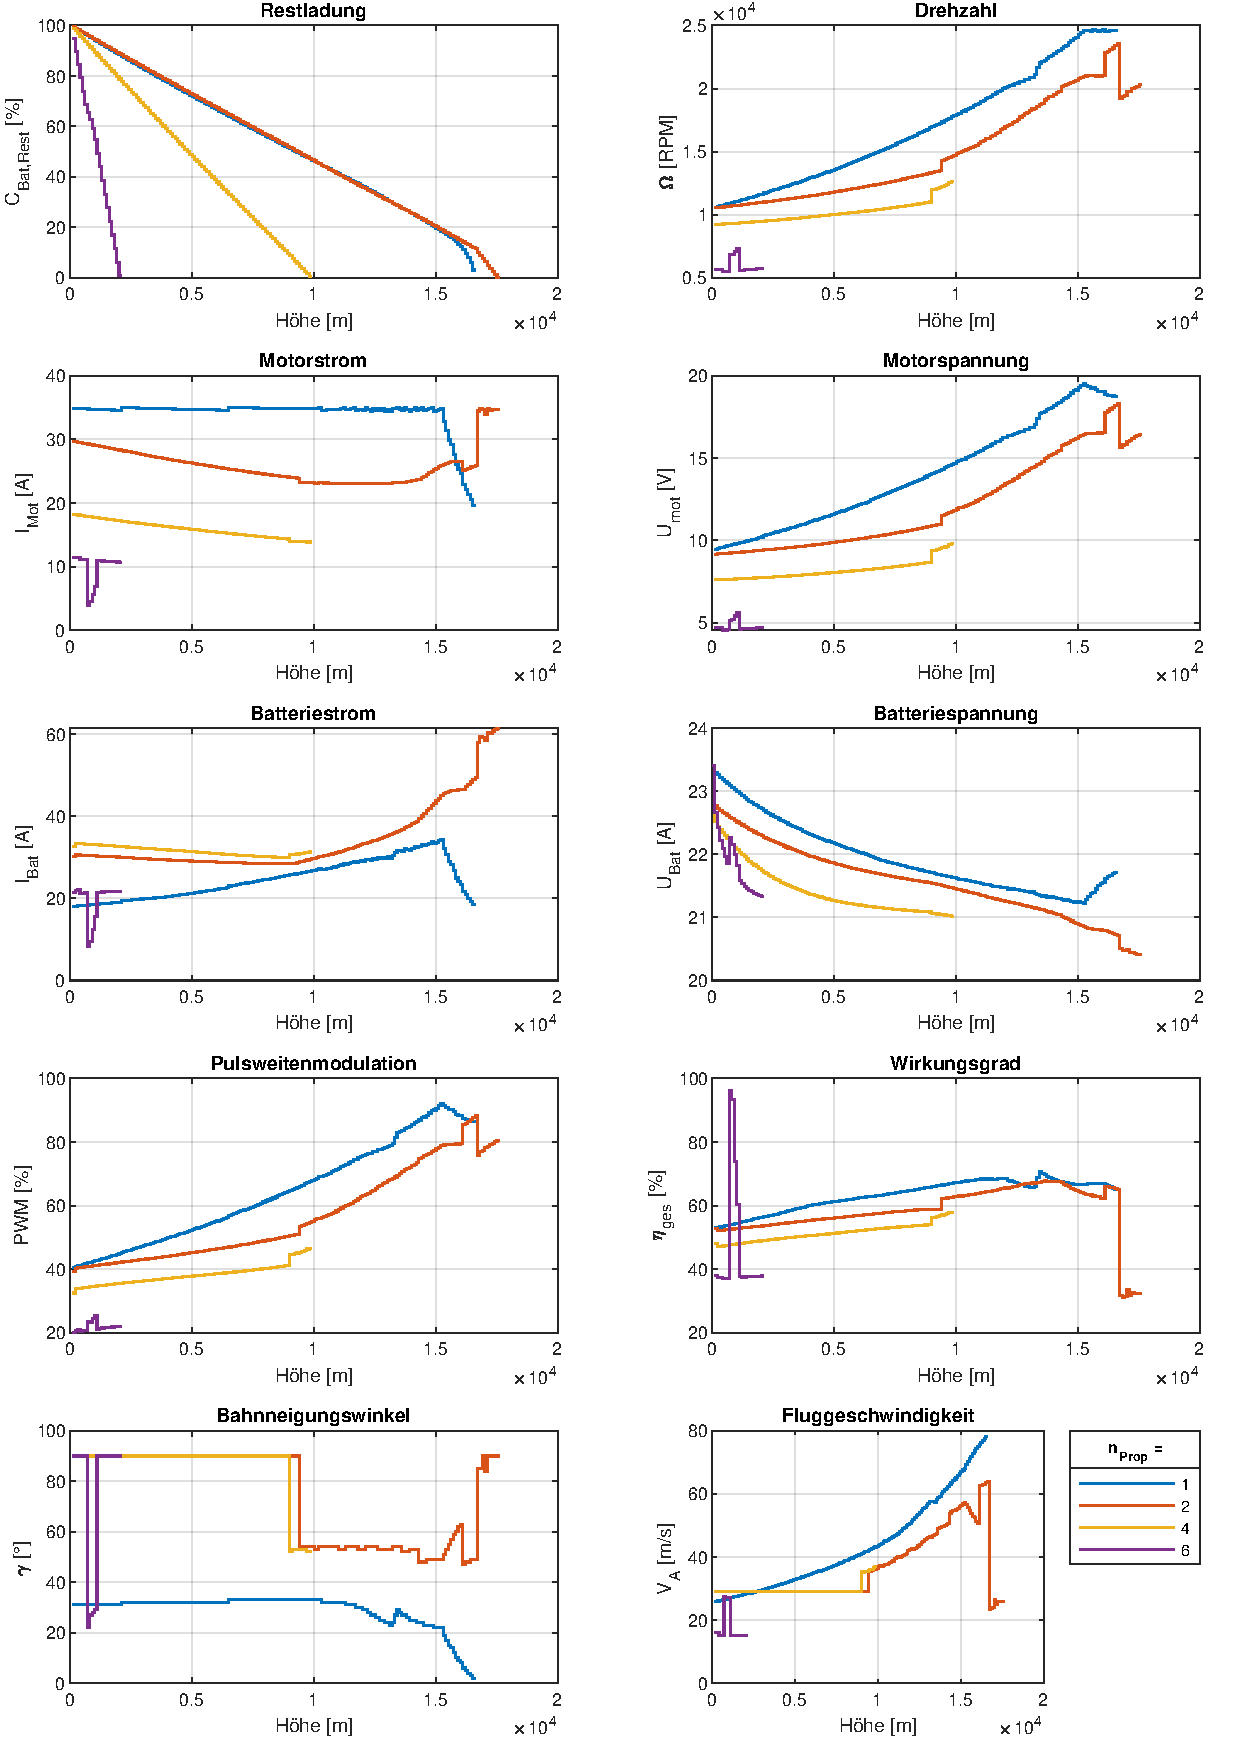
\includegraphics[scale=0.7]{Diagramme/Flaechenflzg_n_prop.pdf}
	\caption{Einfluss der Propelleranzahl auf die Flugleistungen der Flächenflugzeug-Referenzkonfiguration (Tab. \ref{tab:referenzkonfiguration})}
	\label{abb:flaechenflzg_n_prop}
\end{figure}


\subsection{Gleitzahl}
\label{subsec:gleitzahl}
Der Einfluss der Gleitzahl äußert sich hauptsächlich in der Effizienz des Flächenflugzeugkonfiguration, die wiederum durch die Abnahme der Restladung ausgedrückt wird (vgl. Abb. \ref{abb:gleitzahl})
Alle Verläufe erreichen die Dienstgipfelhöhe, die durch die maximale Propellerdrehzahl \ensuremath{\Omega_{Prop}} limitiert wird. Ohne diese limitierende Höhe könnte das Flächenflugzeug bei linearer Extrapolation der Restladungskurve sogar mit einer Gleitzahl von 50 eine Höhe von ca. \SI{25000}{m} erreichen. 
Mit einer Verringerung der Gleitzahl geht auch eine Verringerung der maximalen Höhe mit einher und umgekehrt. Eine entsprechend hohe Gleitzahl bedeutet gleichzeitig auch eine hohe aerodynamische Güte (vgl. \cite[S.34]{Scheiderer.2008}). Dazu sinkt der Widerstand im Vergleich zum Auftrieb, sodass für ein Flächenflugzeug mit einer höheren Gleitzahl (vgl. Gleichung \eqref{eq:gleitzahl}) für den gleichen Auftrieb weniger Leistung zur Kompensation des Widerstandes aufgebracht werden muss. Als Konsequenz dessen steht mehr Leistung für das Steigen zur Verfügung. Mit der Gleitzahl steigt ebenso der optimale Bahnneigungswinkel. Als Grund dafür kann wieder die verringerte Widerstandsleistung angeführt werden. Zusätzlich sinkt die Zeit zum Überwinden einer Höhendifferenz mit einem steileren Winkel. Einen Änderung der Gleitzahl hat nur einen Einfluss auf die Restladung, die Batteriespannung und den Bahnneigungswinkel. Eine geringe Gleitzahl bedeutet einen stärkeren Einbruch der Batteriespannung, da wiederum für den gleichen Auftrieb mehr Widerstand kompensiert werden muss. \\
Auffällig ist noch die Flugleistungsverbesserung mit der Gleitzahl. Diese macht sich im Verlauf der Restladung deutlich bemerkbar. Eine Verbesserung der Gleitleistung von \ensuremath{E = 4} auf \ensuremath{E = 6} bedeutet auf einer Höhe von \SI{15000}{m} bereits \SI{10}{\%} mehr Restladung und einen \SI{7}{^\circ} höheren Bahnneigungswinkel. Eine erneute Erhöhung der Gleitzahl auf 10 steigert die Restladung auf dieser Höhe über dem  Meereslevel nur noch um \SI{5}{\%} und eine Erhöhung des Bahnneigungswinkel \SI{5}{^\circ}. Dieser Trend der abnehmenden Flugleistungsoptimierung bei einer gleichzeitigen Verdoppelung der Gleitleistung setzt sich fort (siehe \ref{abb:gleitzahl}).
Das einfache Flächenflugzeugmodell berücksichtigt nicht, dass eine Gleitzahlerhöhung auch mit einer deutlichen Erhöhung der Strukturmasse einhergeht, weil die Flugzeugzelle, die Flügelform, das Flügelprofil usw. an die neuen Bedingungen angepasst und verstärkt werden müssen. Dieser Zusammenhang wird beim Vergleich der Gleitleistung eines Segelflugzeugs mit dessen Spannweite deutlich. \\
Dementsprechend ist eine Erhöhung des Penalty-Faktors zwingend erforderlich. Unter Berücksichtigung dieser Zusammenhänge gilt es einerseits die Gleitleistung des Flächenflugzeugs für eine Verbesserung der Flugleistungen zu steigern, dies auf der anderen Seite mit der zusätzlichen Masse der Flugzeugstruktur und dem tatsächlichen Gewinn an Flugleistungen abzuwägen. Es ist zu mutmaßen, dass eine Gleitzahl zwischen 6 und 10 die besten Ergebnisse erzielt.

\begin{figure}[H]
\centering
	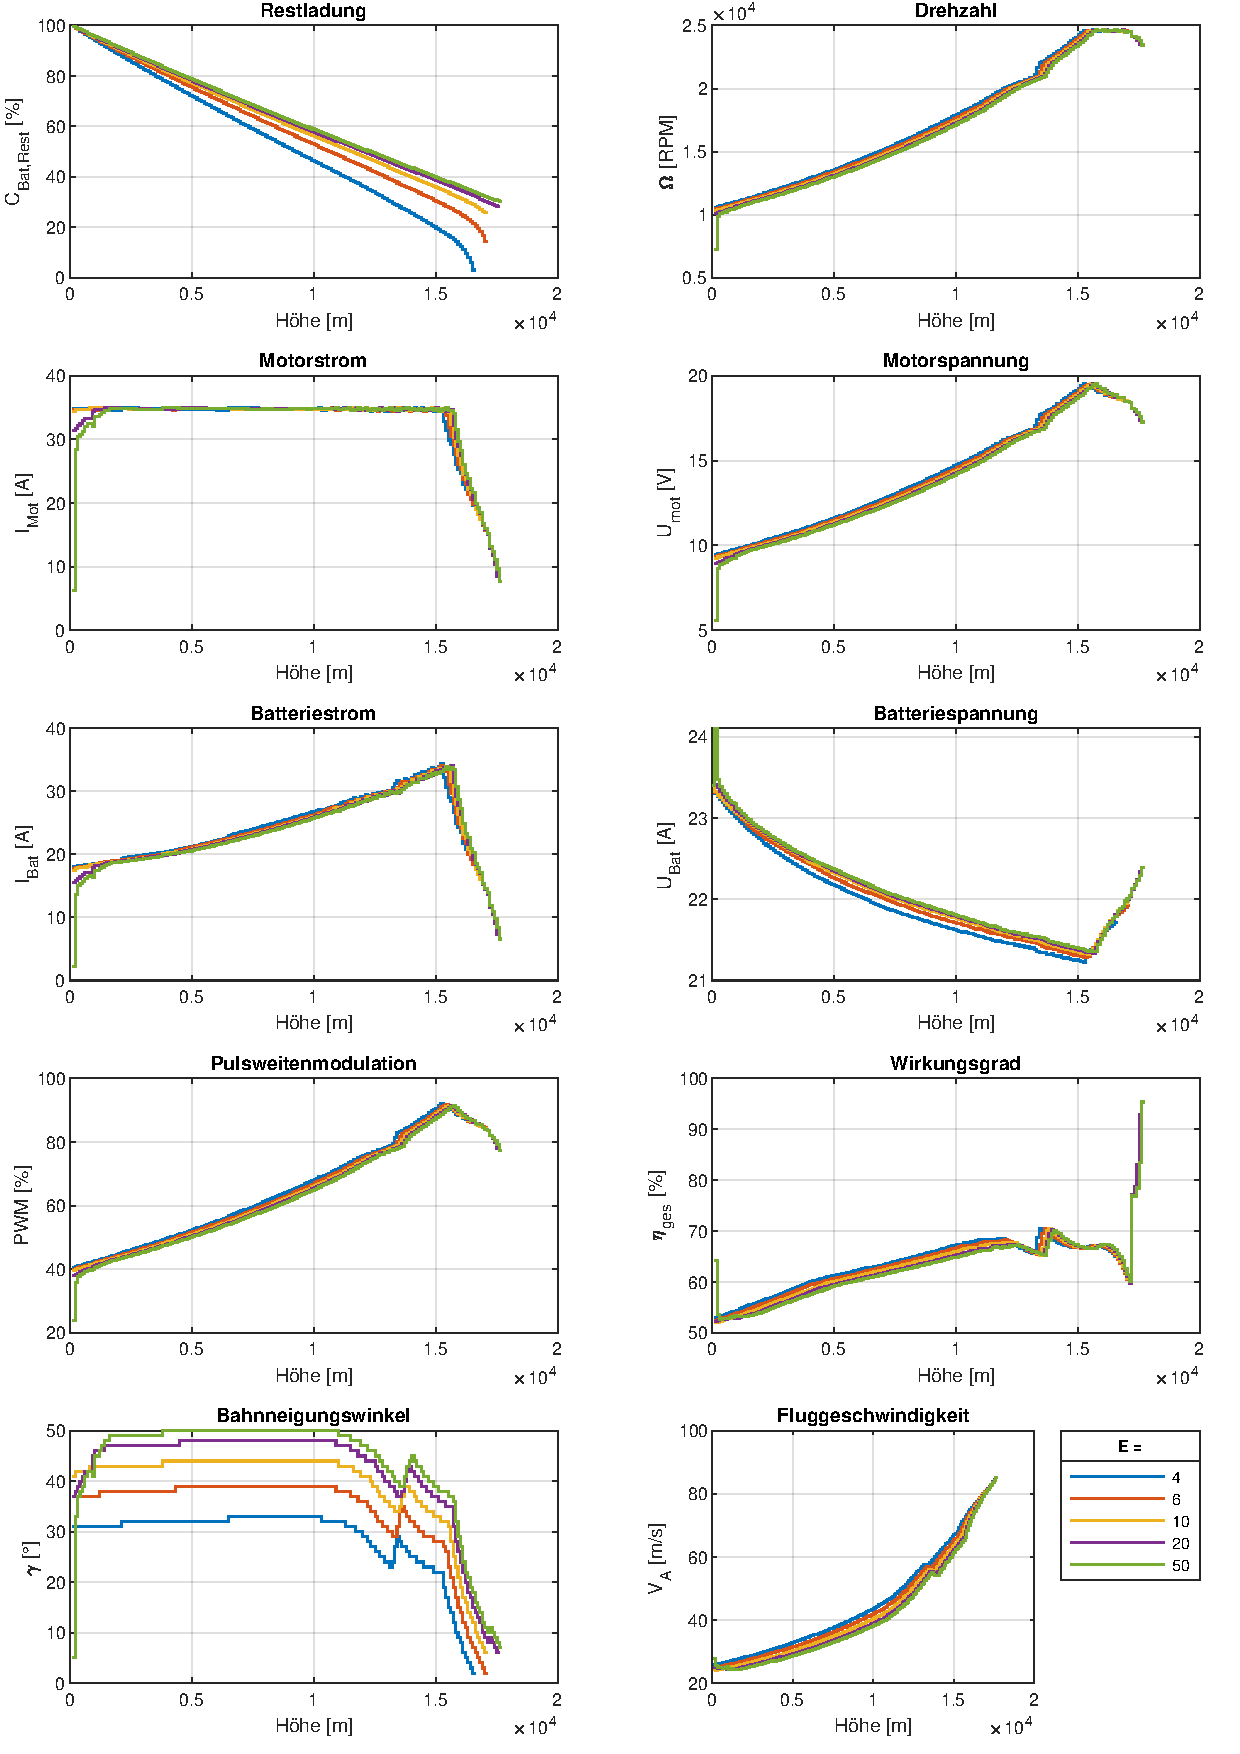
\includegraphics[scale=0.7]{Diagramme/Flaechenflzg_E.pdf}
	\caption{Einfluss der Gleitzahl auf die Flugleistungen der Flächenflugzeug-Referenzkonfiguration (Tab. \ref{tab:referenzkonfiguration})}
	\label{abb:gleitzahl}
\end{figure}


\subsection{Auslegungsgeschwindigkeit}
\label{subsec:vstern}
Die Auslegungsgeschwindigkeit ruft ähnlich zu der Motor-Propeller-Kombination (vgl. Abb. \ref{abb:flaechenflzg_mot_prop}) oder der Propelleranzahl (vgl. Abb. \ref{abb:flaechenflzg_n_prop}) Einflüsse auf das Leistungsverhalten des Flächenflugzeugs hervor. Da für den Steigflug ein Flug mit konstantem Auftriebsbeiwert vorausgesetzt wird, erhöht sich aufgrund dessen die Fluggeschwindigkeit mit der Höhe und größerem Bahnneigungswinkel (vgl. Gleichung \eqref{eq:geschw_flaechenflugzeug}).
Ist die Auslegungsgeschwindigkeit gering, so wächst sie absolut gesehen mit der Höhe nicht so stark wie bei hohen Auslegungsgeschwindigkeiten (vgl. Verlauf der Fluggeschwindigkeit über der Höhe in Abb. \ref{abb:vstern}). 
Bis zu einem \ensuremath{V^\star} von \SI{75}{km/h} ist die Batterierestladung der limitierende Faktor für die Flughöhe. Ab einer Auslegungsgeschwindigkeit von \SI{100}{km/h}, die auch diejenige der Referenzkonfiguration ist, wird wieder die Dienstgipfelhöhe durch \ensuremath{Ma_{tip} = 1} an der Propellerblattspitze erreicht. Bis zu einer Höhe von \SI{13000}{m} sind auch die Verläufe der Restladung von \ensuremath{V^\star} mit \SI{100}{km/h} und \SI{125}{km/h} identisch. Für alle Auslegungsgeschwindigkeiten ist das Flugverhalten gleich dem aus Abschn. \ref{sec:multicopter_vs_flaechenflugzeug}. Es wird wieder solange mit maximalen Motorstrom geflogen, bis entweder die Restkapazität \SI{0}{\%} oder die Dienstgipfelhöhe durch einen anderen limitierenden Leistungsparameter, in diesem Fall wieder die Propellerdrehzahl, erreicht ist. Durch die höhere Auslegungsgeschwindigkeit und demzufolge auch die höhere Fluggeschwindigkeit (vgl. Gleichung \eqref{eq:geschw_flaechenflugzeug}) kommt es zu einer höheren Propelleranströmgeschwindigkeit. Um trotzdem den gleichen Schub zu erzeugen ist eine höhere Drehzahl notwendig. Mit dem schneller drehenden Propeller steigt auch die Motorspannung (vgl. Gleichung \eqref{eq:motorspannung}), der Batteriestrom und über die Motorspannung auch die PWM. Die gesteigerte Propelleranströmgeschwindigkeit verbessert den Propellerwirkungsgrad und als Konsequenz daraus den Gesamtwirkungsgrad. Daher ist der Gesamtwirkungsgrad für größere Auslegungsgeschwindigkeiten besser. Dies kann auch auf den verbesserten Motorreglerwirkungsgrad bei einer höheren PWM zurückgeführt werden (vgl. Gleichung \eqref{eq:eta_pwm}). Es kann schließlich noch festgehalten werden, dass mit steigender Auslegungsgeschwindigkeit der Bahnneigungswinkel \ensuremath{\gamma} abnimmt, da die Zeit zum Überwinden eines Höhenschritts bei einer höheren Geschwindigkeit und geringerem Bahnneigungswinkel sich kaum ändert. \\
Aufgrund dieser Tatsachen ist das Flächenflugzeug auf einigermaßen hohe Fluggeschwindigkeiten von rund \SI{100}{km/h} auszulegen, um zum einen den Leistungsüberschuss der Motoren ausreichend hoch zu halten und zum anderen die Zeit zum Aufstieg nicht zu vergrößern. Weiterhin wird die Auslegungsgeschwindigkeit durch die Wahl des Propellers beeinflusst. Bei gleichem Durchmesser steigt die optimale Auslegungsgeschwindigkeit mit der Propellersteigung.


\begin{figure}[H]
\centering
	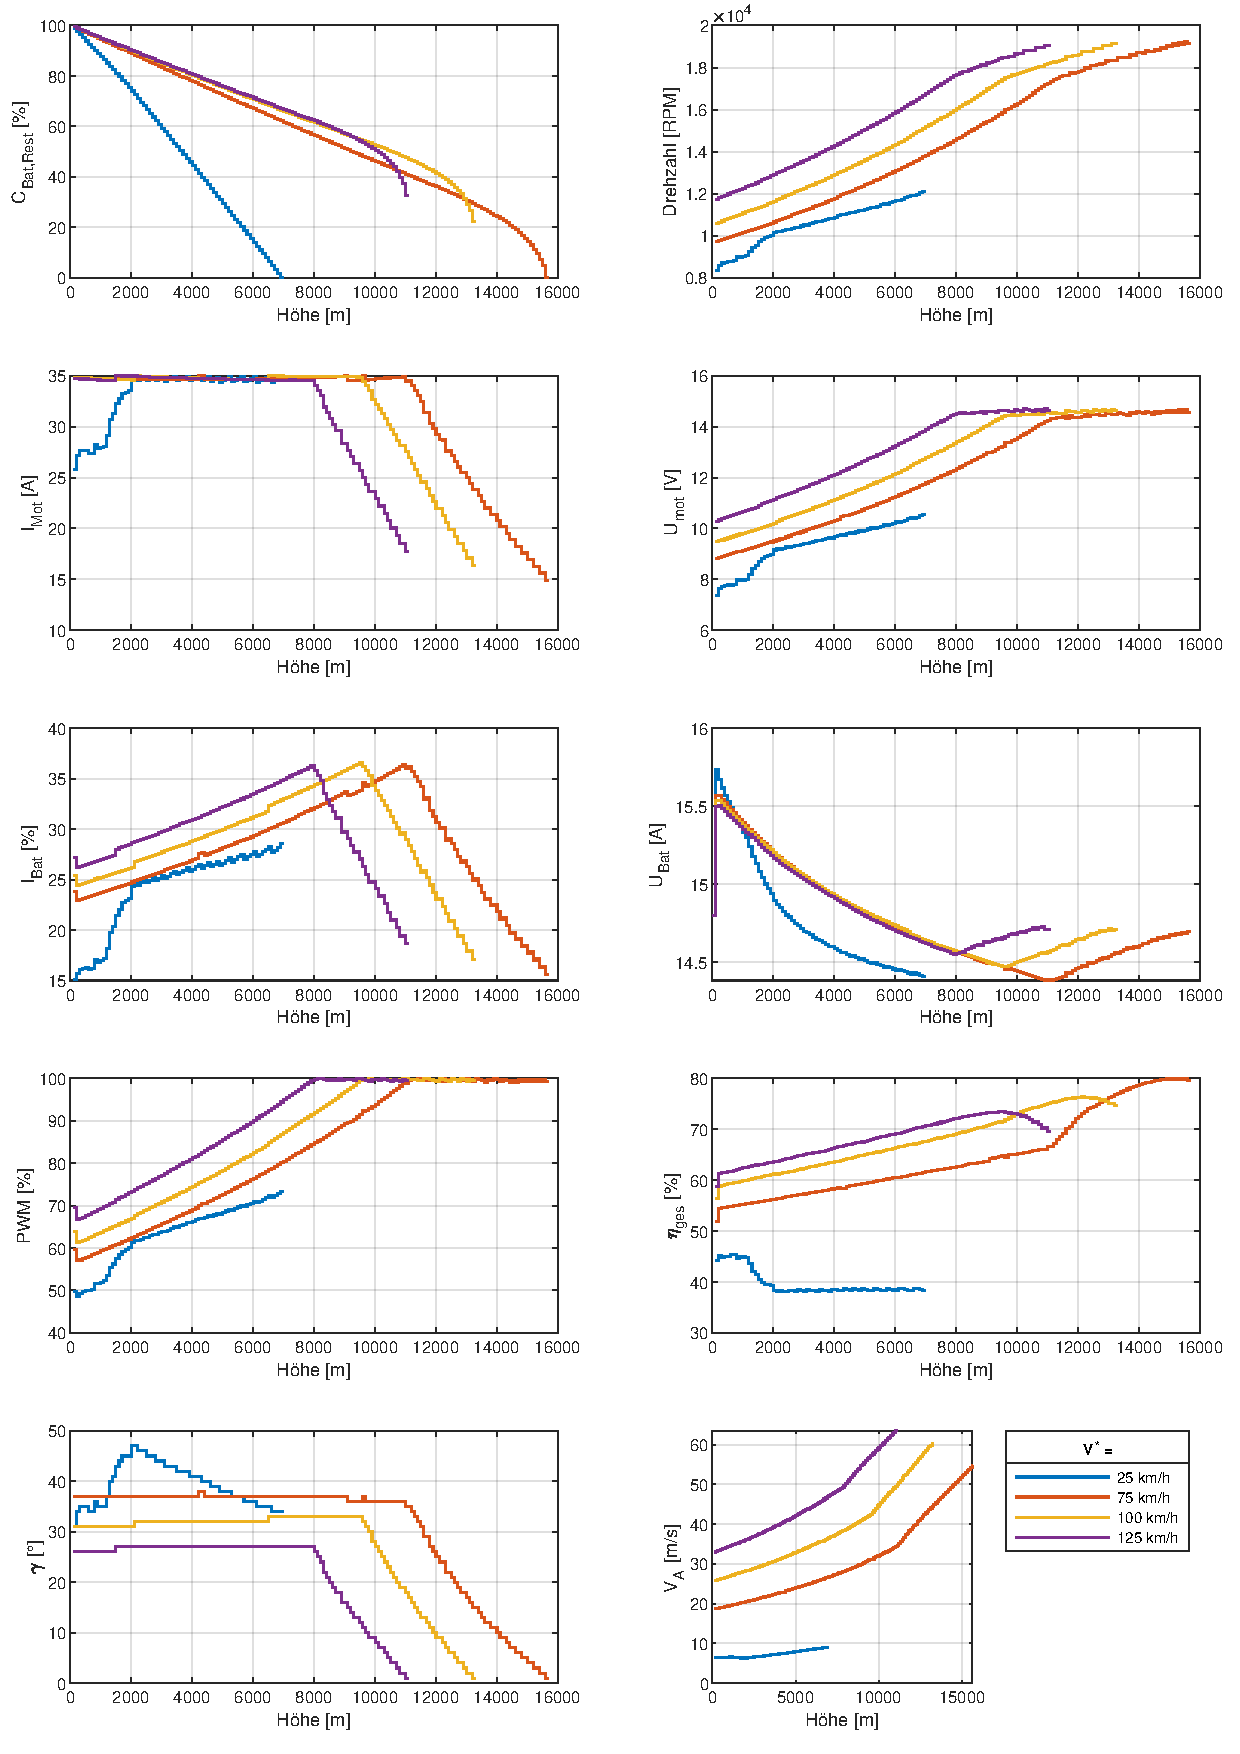
\includegraphics[scale=0.7]{Diagramme/Flaechenflzg_Vstern.pdf}
	\caption{Einfluss der Auslegungsgeschwindigkeit auf die Flugleistungen der Flächenflugzeug-Referenzkonfiguration (Tab. \ref{tab:referenzkonfiguration})}
	\label{abb:vstern}
\end{figure}



\subsection{Penalty-Faktor}
\label{subsec:f_p}
Beim Vergleich von einem Flächenflugzeug mit einem Multicopter muss bei gleichem Gesamtgewicht die unterschiedliche Verteilung der Gewichtskomponenten berücksichtigt werden. Für ein Flugzeug ist das Strukturgewicht von Flügeln und Rumpf sowie den Steuerungselementen bedeutend größer als das von einem Multicopter. Ein Penalty-Faktor von 1 entspricht daher wie oben beschrieben einer optimistischen Einschätzung, wenn beide Strukturgewichte bei einem gleichen Gesamtgewicht äquivalent sind. Um realistischere Ergebnisse für ein Flächenflugzeug zu erreichen, wird der Penalty-Faktor schrittweise erhöht. Dabei verringert sich auch die maximal erreichbare Höhe.
Der Einfluss des Penalty-Faktors konzentriert sich auf die Restladung und die Batteriespannung (vgl. Abb. \ref{abb:fp}). Dies hängt damit zusammen, dass ein Penalty-Faktor größer als 1 die zur Verfügung stehende Batteriemasse (vgl. Gleichung \eqref{eq:penalty}) und folglich die Batteriekapazität (vgl. Gleichung \eqref{eq:batteriekapazitaet}) reduziert. Die Referenzkonfiguration mit \ensuremath{f_P = 1} ist die einzige Konfiguration, die bis zur Dienstgipfelhöhe aufsteigt. Bei allen anderen nimmt die Restladung vorher \SI{0}{\%} an. Die Gesamtmasse ist unabhängig vom Penalty-Faktor identisch für jede Konfiguration, weshalb auch der Schub der gleiche ist und alle übrigen Verläufe der Leistungsparameter identisch sind. 
Aufgrund der Tatsache, dass die Batteriekapazität mit der Batteriemasse abnimmt, der Batteriestrom jedoch gleich bleibt, wird die Entladerate bezogen auf die Kapazität größer (vgl. Gleichung \eqref{eq:c_rate}). Dies ist der Grund für den zunehmenden Spannungsabfall der Batterie bei einem höheren Penalty-Faktor.\\
Insbesondere in Bezug auf Abschn. \ref{subsec:gleitzahl} ist der Penalty-Faktor von Bedeutung. Einer Anpassung der Flächenflugzeugzelle in Richtung einer Flugleistungsverbesserung sind Grenzen gesetzt. 


\begin{figure}[H]
\centering
	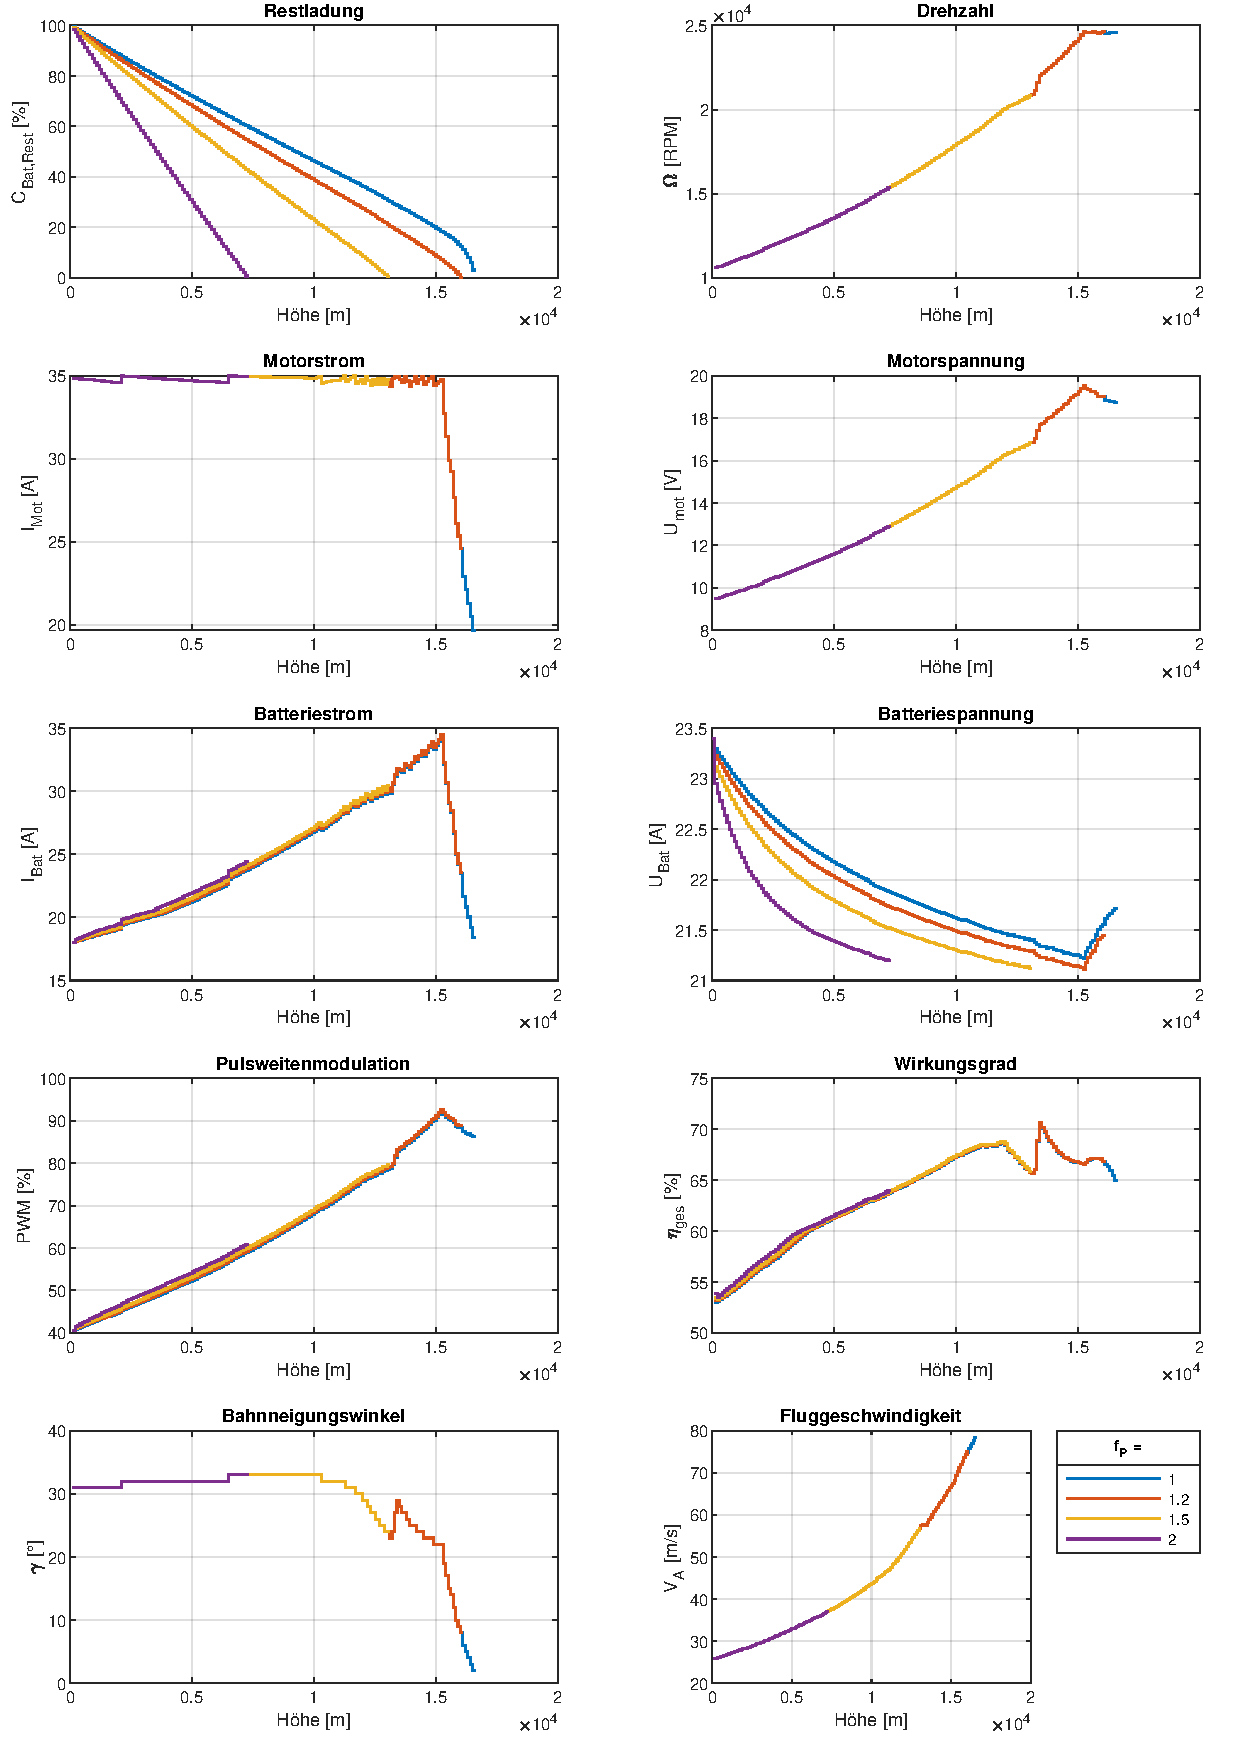
\includegraphics[scale=0.7]{Diagramme/Flaechenflzg_fp.pdf}
	\caption{Einfluss des Penalty-Faktors auf die Flugleistungen der Flächenflugzeug-Referenzkonfiguration (Tab. \ref{tab:referenzkonfiguration})}
	\label{abb:fp}
\end{figure}

\subsection{Zusammenfassung}
Aus den Ergebnissen wird ersichtlich, dass es viele Einflussfaktoren auf die Flugleistungen eines Flächenflugzeug für einen Steigflug auf \SI{10}{km} oder sogar \SI{15}{km} Höhe gibt. Zuerst sollte ein Motor mit einem vergleichsweise hohem \ensuremath{K_V}-Wert in seiner Gewichtsklasse gewählt werden, wobei der Propeller an den Motor anzupassen ist (vgl. Abschn. \ref{subsec:mot_prop_kombi}). Zur Vermeidung transsonischer Effekte sollte der Propellerdurchmesser entsprechend groß gewählt werden, was auch für die Steigung gilt. Die optimale Anzahl der Propeller liegt bei einem oder zwei. Je nach der Propelleranzahl variiert der effizienteste Bahnneigungswinkel, sodass bei einer Propelleranzahl von mindestens zwei das Flächenflugzeug als VTOL-Fluggerät am effizientesten fliegt (vgl. Abschn. \ref{subsec:anz_mot_flaechenflzg}). Weiterhin ist die Gleitleistung so groß wie möglich zu halten (vgl. Abschn. \ref{subsec:gleitzahl}). Hierbei sind einer solchen Erhöhung durch den Penalty-Faktor Grenzen gesetzt (vgl. Gleichung \ref{subsec:f_p}). Die Auslegungsgeschwindigkeit ist an den Propeller anzupassen und so hoch wie möglich zu wählen, um einen Kompromiss aus verbesserter Steiggeschwindigkeit und verringerter Schuberzeugung durch den Propeller zu finden (vgl. Abschn. \ref{subsec:vstern}). In diesem Rahmen ist die Referenzkonstruktion bereits sehr gut ausgelegt.\\


\section{Ergebnisse des Vergleichs}
\label{sec:ergebnisse_vergleich} 
Im direkten Vergleich weist das Flächenflugzeug eine größere maximale Flughöhe (vgl. z.B. Abb. \ref{abb:referenzkonfiguration}) auf als der Quadrocopter aus \cite{Anderson.2018}. Besonders mit hohen Gleitzahlen (vgl. Abschn. \ref{subsec:gleitzahl}), mehreren Motoren (vgl. Abschn. \ref{subsec:anz_mot_flaechenflzg}) und einer guten Kombination aus Motor und Propeller (vgl. Abschn. \ref{subsec:mot_prop_kombi}) wird dieser Vorteil ersichtlich. Jedoch vernachlässigt das einfache Modell des Flächenflugzeugs zusätzliche Widerstände. Die Vorteile eines Flächenflugzeuges zeigen sich auch nur bei einem Penalty-Faktor nahe eins. Dies muss als unrealistisch angesehen werden. Besonders im Bezug auf eine hohe Gleitzahl geht diese Anforderung mit einer hohen Flügelstreckung und damit mit einem hohen Strukturgewicht einher. Somit ist es zwingend notwendig den Penalty-Faktor zu erhöhen. Werden diese Einschränkungen berücksichtigt, schwindet der zusätzliche Höhengewinn eines Flächenflugzeugs gegen Null. Weiterhin erweist sich das Flächenflugzeug als bereits in den möglichen Maßen im Rahmen dieses Modells als optimiert. Die Steiggeschwindigkeit ist in Bezug auf den Auslegungszustand und einem Flug bei Auslegungsgleitzahl optimal. Außerdem wird der Steigwinkel für jeden Höhenabschnitt optimiert (vgl. Abschn. \ref{subsubsec:schub_flaechenflzg}) und eine gute Kombination von Motor und Propeller ist bereits gegeben (vgl. Abschn. \ref{sec:flaechenflugzeug_referenzkonfig}). Schlussendlich ist damit der Spielraum für weitere Verbesserungen eingeschränkt. Ohne die Limitierung durch den Propeller könnte ein  ideales Flächenflugzeug Höhen von mehr als \SI{18000}{m} erreichen. \\
Hingegen zeigt der Quadrocopter in dieser Hinsicht noch Potential. %Ein zu untersuchender Punkt ist noch die Abkehr von einer konstanten Steiggeschwindigkeit hin zu einer kontinuierlichen Optimierung mit der Höhe. %Das Flächenflugzeugmodell aus Abschn. \ref{subsubsec:schub_flaechenflzg} vernachlässigt hier die Abhängigkeit des Flugzeugentwurfs von der Masse. Jede Designänderung verändert die Konstruktion des Flächenflugzeugs z.B. die Struktur und dessen Stärke, das Fahrwerk, den Motor und so weiter. Dieser Zusammenhang findet in dem Flächenflugzeugmodell nur durch die Wahl des Penalty-Faktors Berücksichtigung. \\
Wird für das Flugzeug außerdem eine Konstellation von mehr als einem Motor gewählt, neigt das Flugzeug dazu in einem \SI{90}{^\circ} Winkel zu steigen (vgl. Abschn. \ref{subsec:anz_mot_flaechenflzg}). Damit zeigt sich die optimale Flugweise in einem vertikalen Steigflug. Hierbei werden nichtsdestotrotz wieder viele Vereinfachungen getroffen und Verluste nicht berücksichtigt. 
In der Berechnung der Flächenflugzeugaerodynamik bleibt der Einfluss von Seitenwinden unberücksichtigt, da Seitenwinde nur die Strecke über Grund beeinflussen nicht aber die Flugeigenschaften im Steigflug (siehe Kap. \ref{subsubsec:schub_flaechenflzg}). Unter Berücksichtigung an das angedachte Operationsziel, einer Atmosphärenmessung, sind die Flugkorridore, die von der Deutschen Flugsicherung (DFS) zur Verfügung gestellt werden, begrenzt. Daher ist eine Abdrift bei sehr hohen Seitenwinden für die Mission negativ und muss vom Fluggerät ausgeglichen werden. Dies verbraucht zusätzlich Energie zum Ausgleichen und reduziert nochmals die erreichbare Höhe. Beim Quadrocopter geschieht das bereits durch den Ausgleich der Seitenwinde mit einer Anpassung vom Winkel \ensuremath{\alpha_{M}}, also einer Neigung der Rotorebene. Ein weiteres Argument, was gegen den Einsatz von einem Flächenflugzeug spricht ist, dass eine Start und Landevorrichtung von Nöten ist. Das erfordert Platz für eine Start- und Landebahn. Aufgrund seiner Senkrechtstarterfähigkeit benötigt der Multicopter wenig Platz zum Starten und Landen. 
Entsprechend dieser Argumentation wird in dieser Arbeit entschieden, dass ein Multicopter gegenüber einem Flächenflugzeug für einen Steigflug in die untere Stratosphäre als vorteilhafter anzusehen ist.